
\chapter{Introduction}
\setcounter{page}{1}

Spoken language\index{spoken language} is one of the most powerful system of communication at our disposal. A large part of our waking hours is spent in social interactions mediated through natural language.  The pivotal role of spoken language in our daily lives is largely due to its remarkable proficiency at conveying elaborate thoughts in a robust, flexible and efficient manner. 

Is it possible to exploit this simple observation to develop more human-friendly technologies? Most of our everyday activities are now relying on ``smart'' electronic devices of various kinds, from mobile phones to personal computers and in-car navigation systems. As these technologies gain in autonomy and sophistication, it becomes increasingly important to design user interfaces\index{user interfaces} that can offer rich interactive experiences yet remain easy to use and to adapt. In this context, it seems judicious to endow these devices with a capacity to understand, even in a limited manner, the communication medium that is most natural to us, namely spoken language.  

The ongoing research on \textit{spoken dialogue systems}\index{spoken dialogue dystems} (SDS) is precisely trying to achieve this objective. A spoken dialogue system is a computer agent that is able to converse with humans through everyday spoken language in order to perform its task(s). Such systems are expected to play an ever-increasing role in our daily interactions with technology. They have a wide range of applications, ranging from phone-based systems for information access and service delivery to voice-enabled software for hand-held devices, navigation assistants, interactive tutoring systems, and (in a not-too-distant future) service robots assisting us in our everyday environments.

Figure \ref{fig:basicsds} illustrates an example of interaction between a human user and a spoken dialogue system. When the user starts talking, the system extracts the corresponding speech signal through a microphone.  The speech signal is then processed to analyse its content.  Once this operation is completed, the system must then decide how to react.  In our case, the system decides to greet back the user and selects the words to express it (\utt{good morning, sir}). The final step is then to synthesise these words through an artificial voice, which closes the loop.\footnote{ Needless to say, the schema hides a great deal of internal complexity.  In particular, it omits the existence of non-verbal inputs and outputs (e.g. additional modalities, external actions) which are present in most applications.  The next chapter will describe in more details the software architectures used to design spoken dialogue systems.}

\begin{figure}[h]
\center
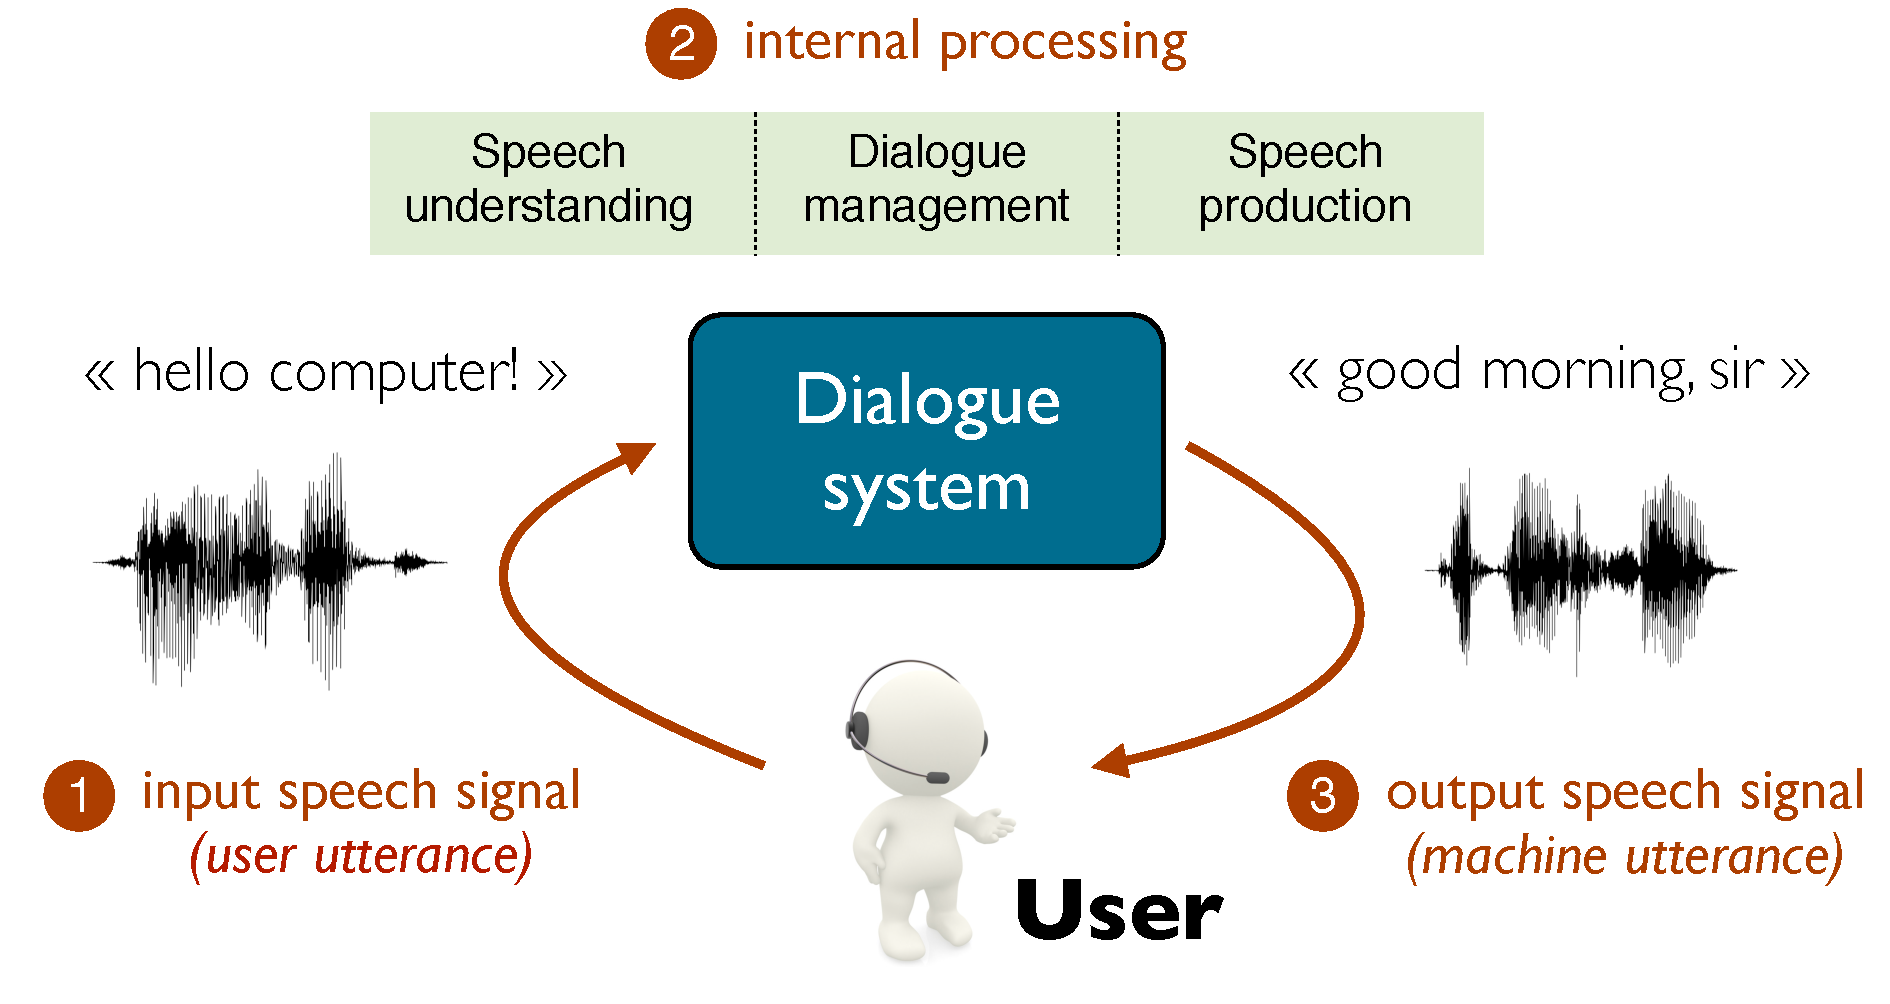
\includegraphics[scale=0.45]{imgs/basicsds.pdf}
\caption{Schematic view of a spoken dialogue system}
\label{fig:basicsds}
\end{figure}

\section{Motivation}

Although the deployment of spoken dialogue systems is attractive for many reasons, their practical development can be a demanding enterprise. Speech is indeed much more complex than other modalities for user interaction such as keyboards or touch screens.  

The present thesis concentrates on the problem of \textit{dialogue management}\index{dialogue management}.  Dialogue management is a central function in spoken dialogue systems.  It serves a double role. 
Its first task is to maintain a representation of the current dialogue state\index{dialogue state}. This representation might include any information that is relevant for the system, and often include features related to the dialogue history, the external context, and the current tasks to perform.  This dialogue state is regularly updated with new information, which comes either in the form of new user utterances or perceived changes in the context. The second task of dialogue management is to make decisions.  Based on the current state of the interaction, dialogue management must decide which actions to undertake. These actions are often communicative in nature (e.g. uttering a sentence), but can also pertain to physical actions to execute (e.g. grasping an object).  

Dialogue management is therefore responsible for controlling the flow of the interaction, by (1) deciding how to interpret the user inputs in their context and (2) selecting which actions to perform next. In the example from Figure \ref{fig:basicsds}, this step corresponds to the decision of responding to the user utterance \utt{hi there!} with another greeting action, \utt{good morning, sir}. 

Along with speech recognition, dialogue management has proven be be one of the most difficult computational problem in spoken dialogue systems. To understand why this is the case, it is useful to have a closer look at two defining features of verbal interactions:
\begin{enumerate}
\item Verbal interactions are highly \textit{complex}.   Understanding a dialogue requires tracking a multitude of factors that evolve over time, such as the history of utterances, the hypothesised goals and preferences of the user, and the external situation. Moreover, these factors depend on one another through multiple relations\index{relational structure} straddling the linguistic and extra-linguistic boundaries. Everyday utterances are rife with elliptical constructions, references and implied content that can only be uncovered based on their context. A given utterance is therefore only intelligible within the larger conversational situation that gave rise to it. 

\item Verbal interactions are also crippled with \textit{uncertainties}\index{uncertainty}.  In order to make sense of a given utterance, a conversational agent must face numerous sources of uncertainty, including error-prone speech recognition, lexical,  syntactic and referential ambiguities, partially observable environments, and unpredictable interaction dynamics.  
\end{enumerate} 

The combination of these two properties forms an explosive mix.  In order to make sense of the interaction and act appropriately, the dialogue system must be able to perform sophisticated reasoning in order to interpret the user intentions in its context and plan the best course of action.  And it must do so under high levels of noise and uncertainty, where many pieces of information can be erroneous, missing, ambiguous, or fragmentary. This task is known in Artificial Intelligence\index{Artificial Intelligence} as \textit{sequential decision-making under uncertainty}\index{sequential decision-making under uncertainty} \citep{Kaelbling:1998,aima2010}, and is known to be a particularly difficult (and often intractable) computational problem, especially for complex domains such as dialogue. 

Research on dialogue management can be divided into two main lines of investigation that reflect their focus on either of the two challenges we just mentioned.  

On the one hand, structural complexity is often dealt with conceptual tools borrowed from formal logic\index{formal logic}.  These approaches provide principled methods for the interpretation and generation of dialogue moves through logical reasoning on the basis of a formal representation of the mental states of the dialogue participants (including their shared knowledge). This representation might incorporate the beliefs, desires and intentions\index{Belief-Desire-Intention model} of each agent \citep{Cohen1979,Allen1980}, social obligations \citep{Traum:1994}, or open questions raised during the interaction \citep{larsson2002,Ginzburg2012}.  These approaches can provide detailed analyses of various dialogue behaviours, but they generally assume complete observability of the dialogue context and provide only a very limited account (if any) of errors and uncertainties. In addition, they require the knowledge base on which the inference is grounded to be completely specified in advance by domain experts.  Their deployment in practical applications is therefore non trivial. 

On the other hand, the problem of uncertainty is usually addressed by probabilistic modelling\index{probabilistic modelling} techniques \citep{Roy:2000,FramptonL09,Young:2010}.  The state of the dialogue is here represented as a probability distribution over possible worlds.  This distribution represents the system's current knowledge of the interaction and is regularly updated as new observations are collected. These probabilistic models provide an explicit account for the various uncertainties that can arise during the interaction. They also enable the dialogue behaviour to be automatically optimised in a data-driven manner instead of relying on hand-crafted mechanisms.  Dialogue strategies can therefore be adapted to new environments or users without having to be reprogrammed. However, these models typically depend on large amounts of training data to estimate their parameters -- a requirement that is hard to satisfy for most dialogue domains.  In addition, the probabilistic models are usually limited to a handful of state variables and are difficult to scale to domains featuring rich conversational contexts. 

The work described in this thesis aims at reconciling these two strands of research through a new, hybrid framework for computational dialogue modelling. 

\section{Contributions}

The present thesis details an original approach to dialogue management based on \textit{structured probabilistic modelling}.  The overarching objective of this work is to design probabilistic models of dialogue that are scalable to rich conversational domains, yet only require small amounts of training data to estimate their parameters.

There is an extensive body of work in the machine learning and decision-theoretic planning literature which shows how to address this issue by relying on more expressive representations, able to capture relevant aspects of the problem \textit{structure} in a compact manner. By taking advantage of hierarchical or relational abstractions, system developers can leverage their domain knowledge to yield probabilistic models which are both easier to learn (due to a reduced number of parameters) and more efficient to use (since the structure can be exploited by the inference algorithm).

This thesis demonstrates how to translate these insights into dialogue modelling\index{dialogue modelling}. We present a new framework for describing probabilistic models of dialogue, based on the concept of \textit{probabilistic rules}\index{probabilistic rules}.  These rules express the distributions in terms of structured mappings associating specific conditions on a set of input variables to probabilistic effects defined on a set of output variables. 

The presented modelling framework offers two major benefits. Most importantly, the reliance on more expressive representations can drastically reduce the number of parameters associated with the models.  Instead of being encoded through traditional probability tables, the conditional distributions between states variables are expressed through high-level rules that capture the dependencies with a compact set of parameters (one for each possible effect). As a consequence, these models are much easier to learn and generalise to unseen data. 

In addition, the framework enables expert knowledge\index{expert knowledge} to be directly incorporated into the probabilistic models. System developers are thus free to exploit powerful abstractions to encode their prior knowledge\index{prior knowledge} of the dialogue domain in the form of pragmatic rules, generic background knowledge, or task-specific constraints.  While there exists previous work on the integration of expert knowledge using finite-state policies or ad-hoc constraints \citep{heeman2007,williams2008}, these approaches essentially use this information source as an external filter to a classical model.  By contrast, our approach incorporates this expert knowledge in the very structure of the statistical model.

At runtime, these probabilistic rules are instantiated on the variables that compose the dialogue state.  This instantiation is realised by converting the rules into the nodes of a Bayesian Network\index{Bayesian Network} (a.k.a. a directed graphical model).  The probabilistic rules can therefore be seen as providing high-level templates for the construction of a classical probabilistic model.  After grounding the rules in the Bayesian Network, various inference operations can be triggered to e.g. update the model with new observations or search for the action yielding the highest utility.  

We conducted several experiments to assess the validity of our approach in different learning scenarios: \begin{enumerate}
\item The first experiment, detailed in Section \ref{sec:wozlearning-experiments}, focussed on the problem of estimating the utilities of various system actions given a small data set collected from Wizard-of-Oz interactions\index{Wizard-of-Oz interaction}.\footnote{A Wizard-of-Oz interaction is an experimental procedure borrowed from Human-Computer Interaction (HCI) studies \citep{woz93}. In a Wizard-of-Oz experiment, the subjects are asked to interact with a computer system which has all the appearances of reality, but is actually remotely controlled by an (unseen) human agent operating behind the curtains.  Wizard-of-Oz studies are often conducted to provide the system designers with interaction data from real users before the system is fully implemented.}  Based on dialogue models encoded with probabilistic rules, the utilities of the different actions were learned through the systematic application of Bayesian inference\index{Bayesian inference} in a supervised learning\index{supervised learning} setting.  We were then able to show that the rule structure enabled the learning algorithm to converge faster and with better generalisation performance than unstructured models. This work was originally presented in \citep{rulebasedmodels-sigdial2012}.
\item The second experiment, described in Section \ref{sec:rllearning-experiments}, extended the above approach to reinforcement learning\index{reinforcement learning}. The goal of this study was to estimate the transition model of the domain from interactions with a user simulator. We compared the relative learning performance of two modelling approaches: one relying on unstructured distributions, and one based on probabilistic rules. The empirical results demonstrated once more the benefits of capturing the domain structure with probabilistic rules. The results were first published in \note{XXX} 
\item Finally, the third experiment was designed to evaluate the approach through live interactions with real users\index{user evaluation}. \note{to be completed}  
\end{enumerate}

An additional contribution of our thesis is a software toolkit that implements all the representations and algorithms presented in this work. The toolkit is dubbed \opendial  and is freely available under an open source licence.\footnote{The toolkit can be downloaded at \urlsmall{http://opendial.googlecode.com}.} It enables system developers to design, evaluate and deploy dialogue systems based on probabilistic rules. 
The toolkit is fully generic since all all domain-specific knowledge is declaratively specified in the rules for the domain\index{declarative design}.  This design choice effectively simplifies the system architecture to a small set of core algorithms for accessing and updating the dialogue state \citep{lison-semdial2012}. The \opendial  toolkit comes with a user interface allowing developers to interactively test their system and visualise how the internal dialogue state is evolving over time.  Its implementation is described in Appendix \ref{chap:opendial}. 

\begin{wrapfigure}[19]{r}{60mm}
\vspace{-6mm}
\begin{center}
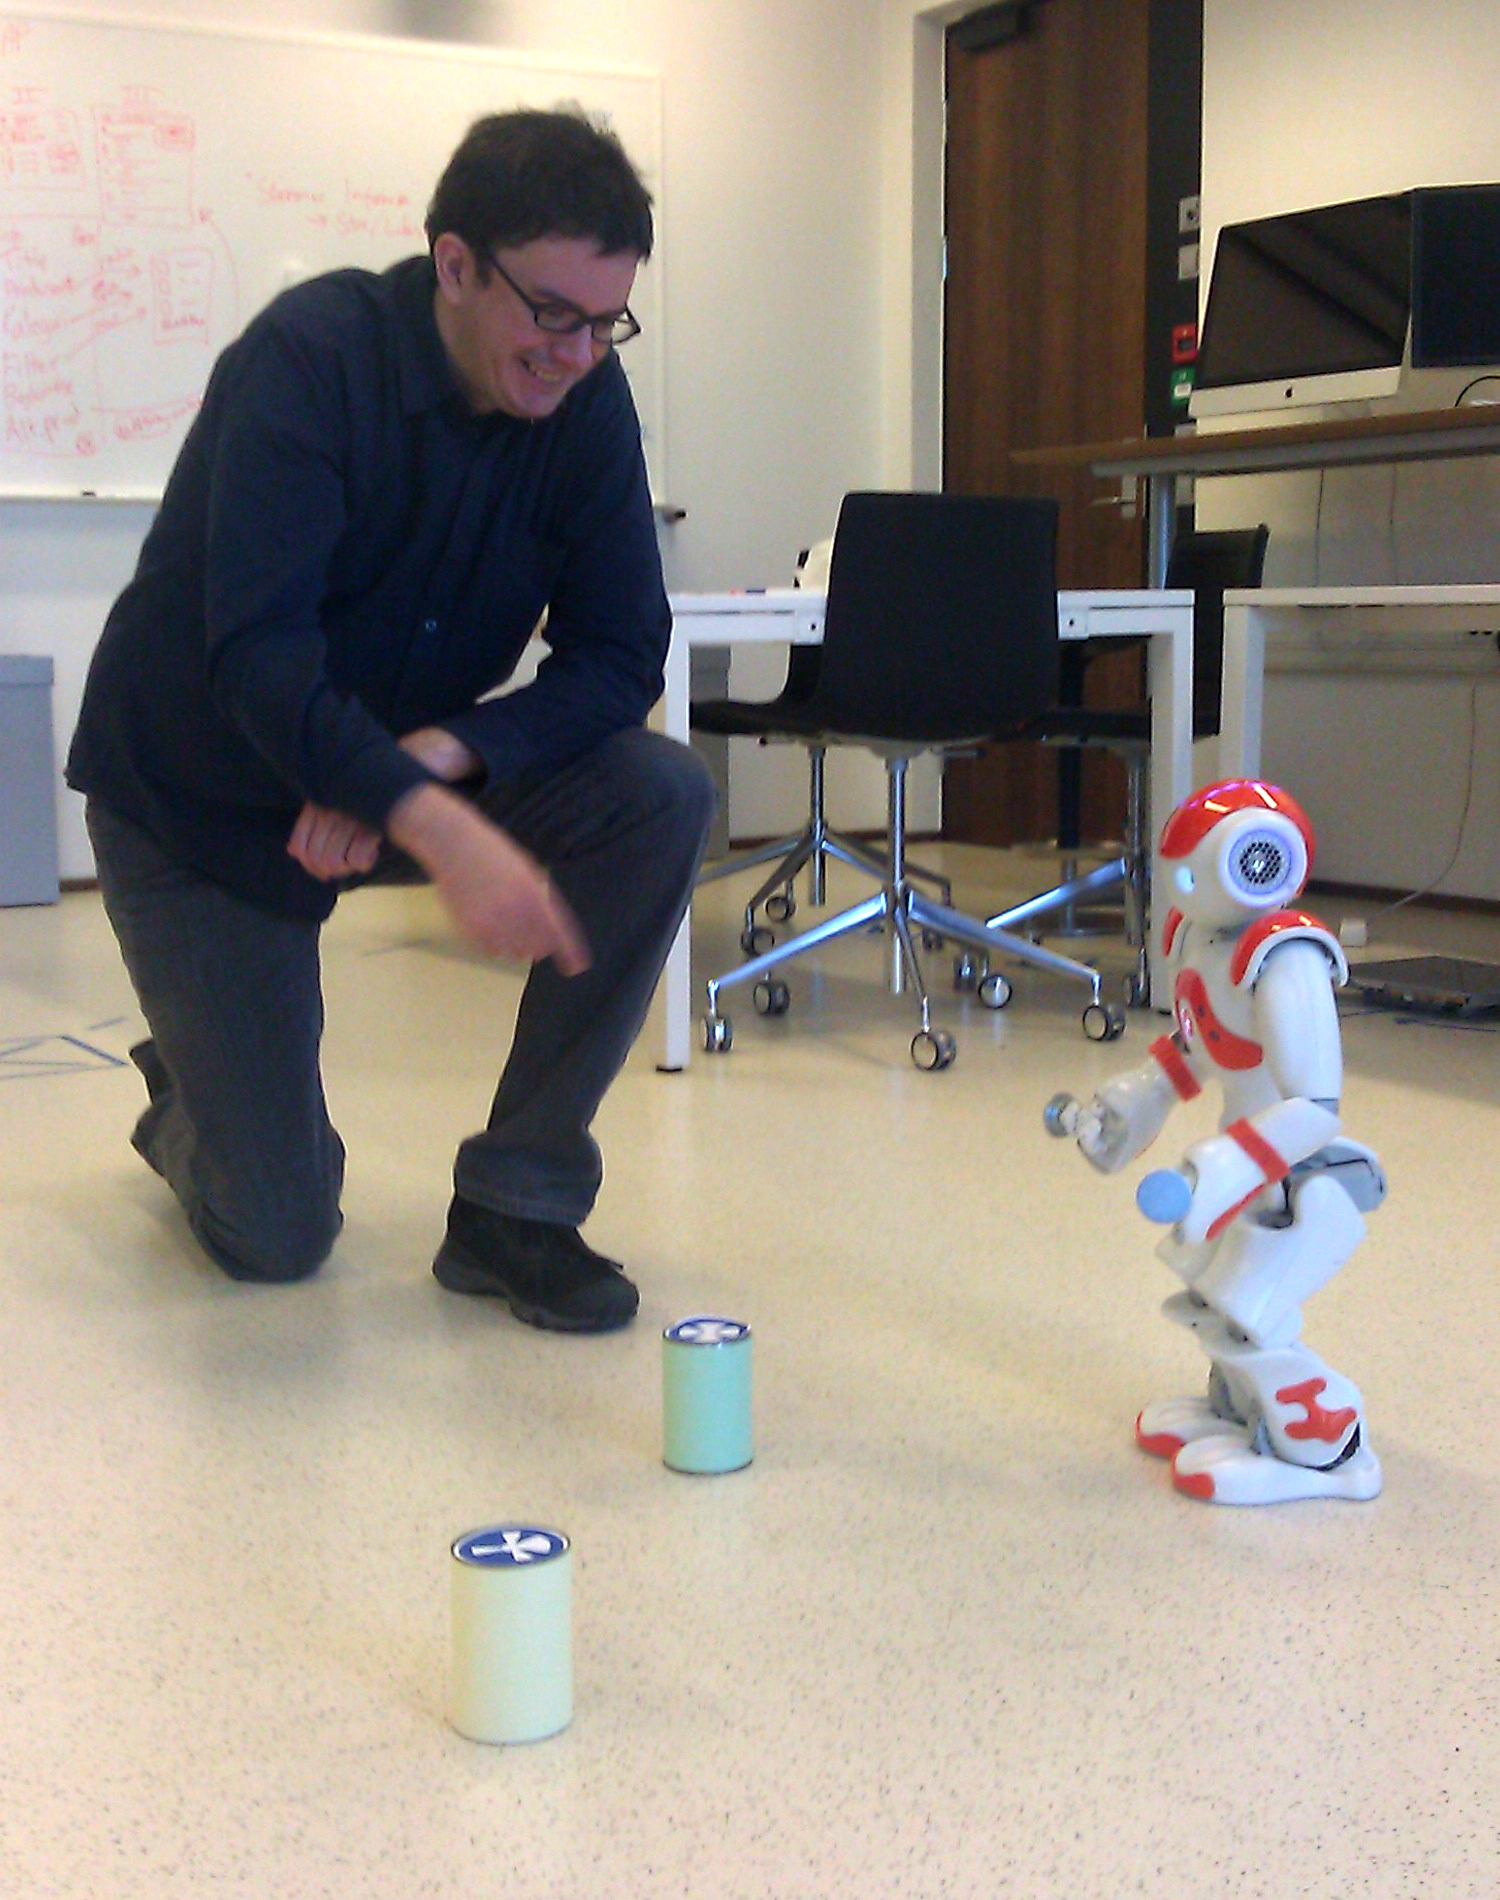
\includegraphics[scale=0.10]{imgs/nao1.jpg}
\end{center} 
\caption{Human user interacting with the Nao robot.}
\label{fig:nao}
\end{wrapfigure}

We carried out all the experiments described in this thesis in a \textit{human--robot interaction} \index{human--robot interaction} (HRI) domain.  The selection of this application domain as a test bed for our framework was motivated by two factors.  First of all, HRI domains often embody a rich mix of contextual features extracted from the situated environment and the tasks to complete by the agent. Moreover, HRI domains must frequently significant levels of uncertainty due to imperfect sensors, unreliable motors, and failure-prone speech recognition. 

The Nao robot\index{Nao robot} from Aldebaran Robotics was used as a platform for all our experiments.\footnote{cf.  \urlsmall{http://www.aldebaran-robotics.com}.}  An example of interaction with the robot is shown in Figure \ref{fig:nao}.  Most of our experiments involved the Nao robot interacting with a human user in a shared visual environment featuring a few basic objects that can be automatically perceived by the robot.  The user were instructed to command the robot to execute various tasks such as grasping objects and moving them from one place to the other.  The robot was also able to answer questions related to his own perception (e.g. \utt{do you see the red cylinder?}).  A detailed description of the experimental setup is provided in the Chapters 4--6. 

\section{Outline of the Thesis}

We provide here a brief outline of the thesis structure, chapter by chapter. 

\begin{description}
  \item[\textbf{Chapter \ref{chap:background}: Background}] \hfill  \vspace{2mm}
  
This chapter introduces the fundamental concepts and methods used throughout this thesis. We start with an overview of some of the core linguistic properties of dialogue and describe key notions such as turn-taking, dialogue acts and grounding.  We then describe the software architectures used to design spoken dialogue systems and the role of each component within them.  We also mention a range of important applications for spoken dialogue systems. Finally, we survey the various approaches that have been put forward in the research literature to address the dialogue management problem.  In particular, we review both hand-crafted and statistical approaches to the design of dialogue strategies.   \vspace{2mm}

  \item[\textbf{Chapter \ref{chap:rules}: Probabilistic Rules}] \hfill \vspace{2mm}
 
  This chapter lays down the theoretical foundations of our approach.  We start by reviewing the core notions of graphical models, since they constitute the formal basis for our framework. We then define what probabilistic rules are and how they are internally structured through conditions and effects.  We describe two main types of rules, used to respectively encode probability and utility models. Following this, we explain how the rules are practically instantiated in the Bayesian Network representing the dialogue state.  The chapter also addresses some advanced modelling questions, and concludes by discussing related work that also aimed at reducing the dimensionality problem when learning dialogue strategies.  \vspace{2mm}
  
  \item[\textbf{Chapter \ref{chap:wozlearning}: Learning from Wizard-of-Oz data}] \hfill  \vspace{2mm}
  
 This chapter shows how the parameters attached to probabilistic rules can be automatically learned from training data, in a supervised learning fashion. The algorithm to estimate these parameters is grounded in Bayesian inference.  To validate our approach, we detail an experiment showing how to learn the utilities of a set of actions from Wizard-of-Oz data collected in a human--robot interaction domain.  The experiment illustrates in particular the benefits of applying probabilistic rules.  \vspace{2mm}

\item [\textbf{Chapter \ref{chap:rllearning}: Learning from Interactions}] \hfill  \vspace{2mm}

This chapter builds upon the previous chapter and extends it to a reinforcement learning context.  We show that is is possible to efficiently learn the parameters of dialogue models from observations collected during the interaction itself, without having access to any gold standard annotations.  The learning procedure follows a model-based Bayesian reinforcement learning approach. Finally, we report the results of an experiment carried out with a user simulator.  The experiment concentrated on the estimation of the transition model in a HRI domain, and evaluated the relative performance of a  model structured with probabilistic rules compared to a plain probabilistic model.   \vspace{2mm}

\item [\textbf{Chapter \ref{chap:user-evaluation}: User Evaluation}] \hfill  \vspace{2mm}

This chapter presents a user evaluation of our approach in a HRI domain.  \note{XXX}   \vspace{2mm}

\item [\textbf{Chapter \ref{chap:conclusions}: Concluding Remarks}] \hfill  \vspace{2mm}

The final chapter concludes this dissertation with a summary of the presented research contributions, followed by an outline of future work.   \vspace{2mm}

\end{description}

